\part{Qt Framework}

\begin{description}
    \item[Zweck] Erstellung von User Interfaces (im speziellen für GUIs) und plattformunabhängige Anwendungen (im Bereich Desktop, Embedded und Mobile).
    \item[Anwendung] Skype, Google Earth, Wolfram Research und viele mehr.
\end{description}

\section{Qt Oberflächen}
\paragraph{Qt Desktop (Qt Widgets)}
Qt Oberflächen basieren auf der Qt C++ Klassenbibliothek, welche für die GUI-Elemente (``Widgets'') entsprechende Klassen wie QLabel, QPushButton etc. bereitstellt. Das GUI wird unter Verwendung dieser Klassenbibliothek als C++-Programm geschrieben und häufig für die Maus- und Tastaturbedienung genutzt.
Neben Qt Widget gibt es noch Qt-Quick (QML) und WebEngine. Der Fokus der Vorlesung liegt auf Qt Desktop.

\paragraph{Qt-Quick}
Qt-Quick basiert auf QML (= Qt Meta Language oder Qt Modelling Language), einer speziellen Sprache, welche das Aussehen des Programms festlegt. Verfügt über eine ``Deklarative'' Festlegung der Darstellung und des Verhaltens, ähnlich wie bei HTML mit Javascript. Qt-Qucik wird vielfach für mobile Applikationen mit Touchscreen Bedienung genutzt.

\paragraph{QWebEngine}
Web Engine wird für die Darstellung von Web Content mit HTML/CSS/JS verwendet.

\section{Namenskonventionen}
\begin{description}[leftmargin=*,widest={\textbf{Q\_BIG}}]
    \item[Qt\textit{Module}] QtCore Hauptmodul (wird von allen Modulen genutzt); Weitere Module: QtGui, QtWdigets, QtNetwork, QtSql, QtTest
    \item[Q\textit{Class}] Klasse wie QObject, QApplication, QWidget, QDialog, QString
    \item[q\textit{Foo}] globale Variable / Funktionsname wie \lstinline{qApp, qTranslator, qDebug(), qWarning(), qFatal()}
    \item[Q\_\textit{BIG}] Qt-Makro-Namen wie \lstinline{Q_OBJECT, QCOMPARE, QEXPECT_FAIL, QFETCH}
    \item[Header] \lstinline{#include <QtModule>} wie \lstinline{#include <QtGui>}, \lstinline{#include <QObject>} oder \lstinline{#include <QString>}
\end{description}

\section{Meta Object System}
Dieses System bietet zusätzliche Funktionaitäten zu C++. Es unterstützt das Hollywood Prinizip mittels \emph{Signals and Slots}. Es basiert auf QObject Klassen, \lstinline{Q_OBJECT} Makro und einem Meta-Object Compiler (moc).

\subsection{QObject}
Aus der QObject Klasse wurden weitere Qt Klassen abgeleitet wie z.B. QPushBotton, QLabel, QGridLayout, QTimer und QThread. Die QObject Klasse wird zu einem header file hinzugefügt mit \lstinline{#include <QObject>}. QObjects können mit einer Parent-Child-Beziehung verknüpft werden, woraus ein ganzer QObject Tree entstehen kann. Ein Object Tree macht es einfacher eine grosse Anzahl an Dokumente, die miteinander verbunden sind, auf einen Schlag zu löschen.
Das Eltern-QObject wird im C'tor des Child-QObjects wie folgt angegeben:
\begin{lstlisting}
QLabel * child = new QLabel("0000", \&parent);
\end{lstlisting}
Alternativ kann \lstinline{setParent()} verwendet werden: 
\begin{lstlisting}
child->setParent(parent)
\end{lstlisting}

Dies kann jedoch bezüglich der D'tor Reihenfolge problematisch sein (Siehe Prakti 2).
Ein Parent-Object kann beliebig viele child-Objects haben, während ein child-Object nur ein parent-Object hat. Die Löschung eines parent objects hat die automatische Löschung sämtlicher child objects zur Folge. Die Löschung eines child objects zerstört einfach die Beziehung zum parent object. 

\subsection{Meta Object Compiler (moc) \& QMake}
Der Meta Object Compiler (moc) durchsucht das header file nach \lstinline{Q_OBJECT} Makros und generiert ein \texttt{moc\_XXX.cpp} File mit dem meta-object relevanten Code erstellt. Diese Dateien müssen bei der Ausführung zur Anwendung hinzugelinkt werden. Für die Verlinkung und Ausführung von Meta Object Compiler (moc), User Interface Compiler (uic) und Resource Compiler (Rcc) wird qmake verwendet, welche diese Qt Compiler automatisch einbindet. Qmake erzeugt aus einer plattformunabhängigen Projektbeschreibung, dem Projektfile (.pro-Datei) ein plattformspezifisches `Makefile'. Diese Makefile wird dann von den platformspezifischen Tools wie make dazu verwendet, um die Source-Files zu verarbeiten (compilieren, etc.). Dabei ist qmake selbst ein plattformunabhängiger make-file-Generator.
Der Befehl lautet: \texttt{qmake <project file name>.pro}

\begin{figure}[ht]
    \centering
    % \adjustbox{width=12cm}{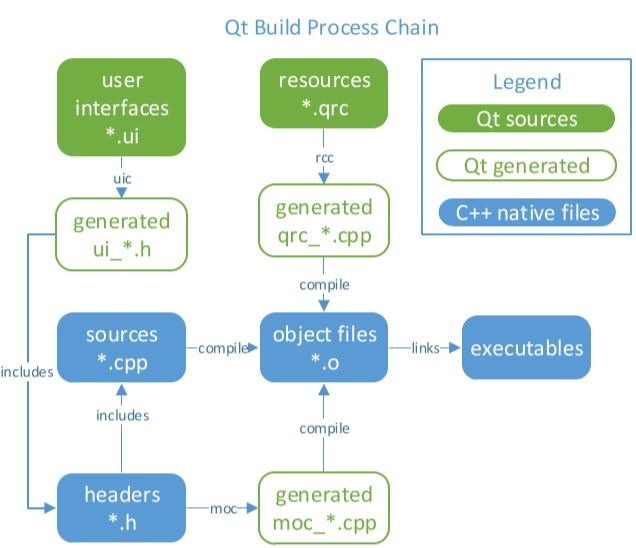
\includegraphics{Figures/qmake}}
    \caption{Qt Build Prozessablauf}
\end{figure}

\subsection{Projektbeschreibung (\texttt{*.pro})}
% TODO: rewrite this
% \begin{multicols}{2}
\textbf{Keywords:} 
- QT: Liste von verwendeten Qt Modulen 
- Target: Name der Applikation (Output File) 
- TEMPLATE: Projekt Typ: app oder lib 
- CONFIG: z.B. CONFIG += C++14  
- windows/linux/macx: Plattform spezifische   Compilierungsregeln 
- SOURCES/HEADER/FORMS: Source-, Header- oder Formdateien die dem Projekt hinzugefügt werden sollen 
% \columnbreak
% FIXME
% \adjustbox{width=6.5cm}{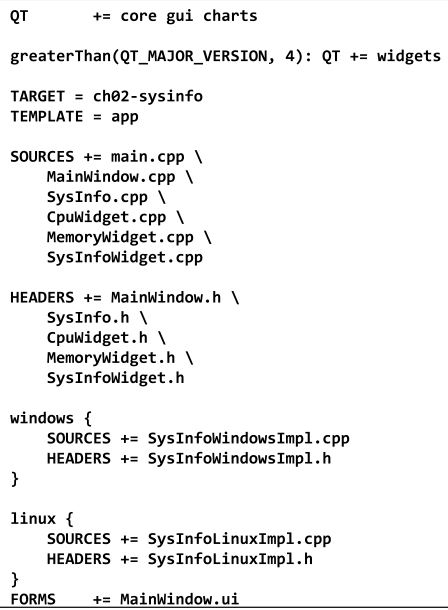
\includegraphics{Figures/keywordspro}}
% \end{multicols}


\section{Hallo Welt Beispiel}

\begin{lstlisting}[language=c++]
#include <QtWidgets>

int main(int argc, char *argv[])
{
    QApplication app(argc, argv);
    // Erstellen eines Textfelds mit dem Text Hello Qt World!
    QLabel label ("Hello Qt World!");
    // Textfeld in der Mitte ausrichten
    label.setAlignment(Qt::AlignCenter);
    // Breite & Höhe des Testfelds
    label.resize(250, 150);
    // Titel des Popup Fenster
    label.setWindowTitle("My first Qt-Program");
    // Befehl zum Anzeigen des Textfelds 
    label.show();

    return app.exec();
}
\end{lstlisting}

\subsection{QApplication Klasse}
Die QApplication Klasse ist pro Qt Applikation nur einmal vorhanden. Sie ist zuständig für das Event handling und weitere Qt Framework spezifische Funktionälitäten. Eine der Methoden heisst \lstinline{exec()}. In dieser Methode verbirgt sich die \lstinline{while(1)} Schleife.
QApplication Klasse ist zudem für die Initialisierung der Applikation mit optionalen Funktionen wie beispielsweise \lstinline{font()} und \lstinline{doubleClickInterval()} zuständig.

\section{Widgets \& Layouts}

\subsection{QWidgets}
Applikation mit GUI = Problem-Domain + Darstellung + Interaktion 
Beispiel: Counter = Funktionalität (inkrementieren und dekrementieren) + Fenster mit inc \& dec Buttons und der Anzeige des aktuellen Counter-Stands + Inkrementieren, wenn inc-Button gedrückt.

\paragraph{Allgemeine Konzepte von GUI Frameworks}
\begin{itemize}
    \item \textbf{Ansicht festlegen} Visuelle Elemente in der Benutzeroberfläche werden mittels Klassen vom GUI Framework zur Verfügung gestellt. 
    \item \textbf{Interaktion} mit dem Programmbenutzer \(\rightarrow\) Signals \& Slots
\end{itemize}

\subsection{QWidget Klasse}
QWidget (Widget = "Window Gadget") ist eine Basisklasse für alle anderen Qt Widgets wie bspw. QLabel, QLineEdit, QPushButton
QWidget übernimmt als Parent-Widget folgende Aufgaben:
\begin{itemize}
    \item Anzeigen, verstecken, freigeben, sperren \(\rightarrow\) wird auch auf die Child-Widgets angewendet 
    \item Weiterleiten von Ereignissen an die betroffenen Child-Widgets
    \item Memory Management 
\end{itemize}

\begin{figure}[hb] \centering
    % FIXME
    % \adjustbox{width=7.5cm}{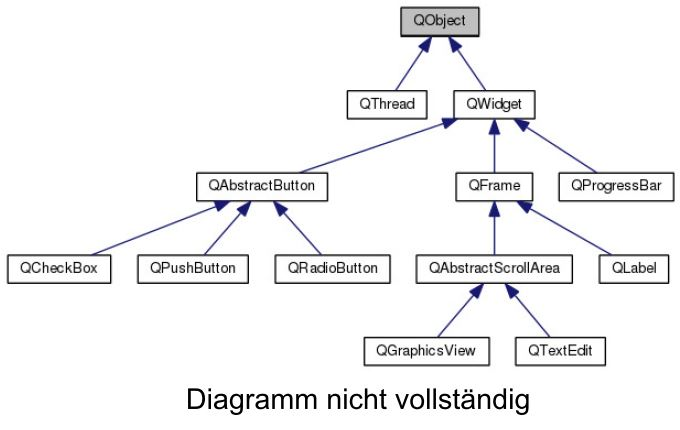
\includegraphics{Figures/qtwidgets_objekte}}
    \caption[]{Qt Vererbungen von QObject und QWidget}
\end{figure}

\subsection{Layout}

\begin{table}[h] \centering
\begin{tabular}{lll}
    \toprule
    Art          & Selbst codiertes GUI             & GUI-Designer (Qt Creator)    \\
    Beschreibung & C++ Code für GUI Beschreibung    & Interaktives Tool            \\
    Vorteil      & kann sich zur Laufzeit ändern    & schnell zusammen "geklickt"  \\
    Nachteil     & aufwändig, Code selber schreiben & Nur statische Design möglich \\
    \bottomrule
\end{tabular}
\end{table}

Bei der Erstellung eines GUIs mittels WYSIWYG Editor – GUI-Designers (Qt-Creator) erfolgt die Anordnung der Widgets innerhalb eines sogenannten Formulars mit Hilfe eines interaktiven Tools. Es erfolgt eine automatische Umwandlung der Formulardaten (\texttt{*.ui}) in entsprechenden Programmcode mittels uic.

\subsection{Manuelles Layout}

\begin{figure}[ht]
    \centering
    % \adjustbox{width=0.8\textwidth}{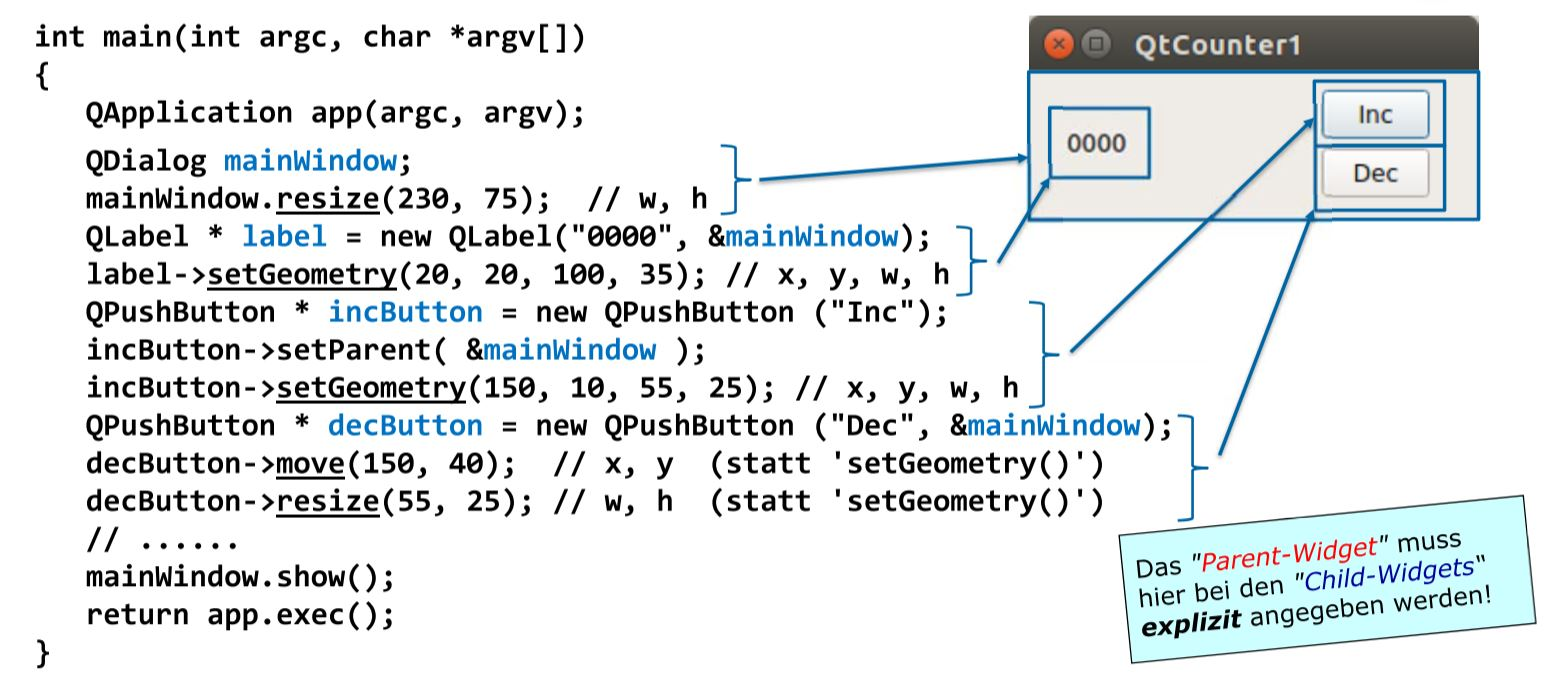
\includegraphics{Figures/Layout}}
    \caption[]{Beispeil eines manuellen Layouts}
\end{figure}

Die Positionierung erfolgt mittels eines Koordinatensystems bei dem der Ursprung (0,0) in der linken oberen Ecke ist. Die Position und Grösse wird in Pixel angegeben. Die x-Werte erhöhen sich nach rechts, während die y-Werte nach unten ansteigen. (x, y) sind die Koordinaten der linken oberen Ecke eines Widgets innerhalb eines anderen, des äusseren Widgets. w, h sind Breite und Höhe des inneren Widgets.

Methoden zur Festlegung von Position und/oder Grösse
\begin{lstlisting}[language=c++]
void QWidget::setGeometry(int x, int y, int w, int h);
void QWidget::resize (int w, int h);
void QWidget::setFixedSize(int width, int height);
void QWidget::move (int x, int y);
\end{lstlisting}

\section{Layout Manager}
\begin{figure}[ht]
    \centering
    % \adjustbox{width=0.7\textwidth}{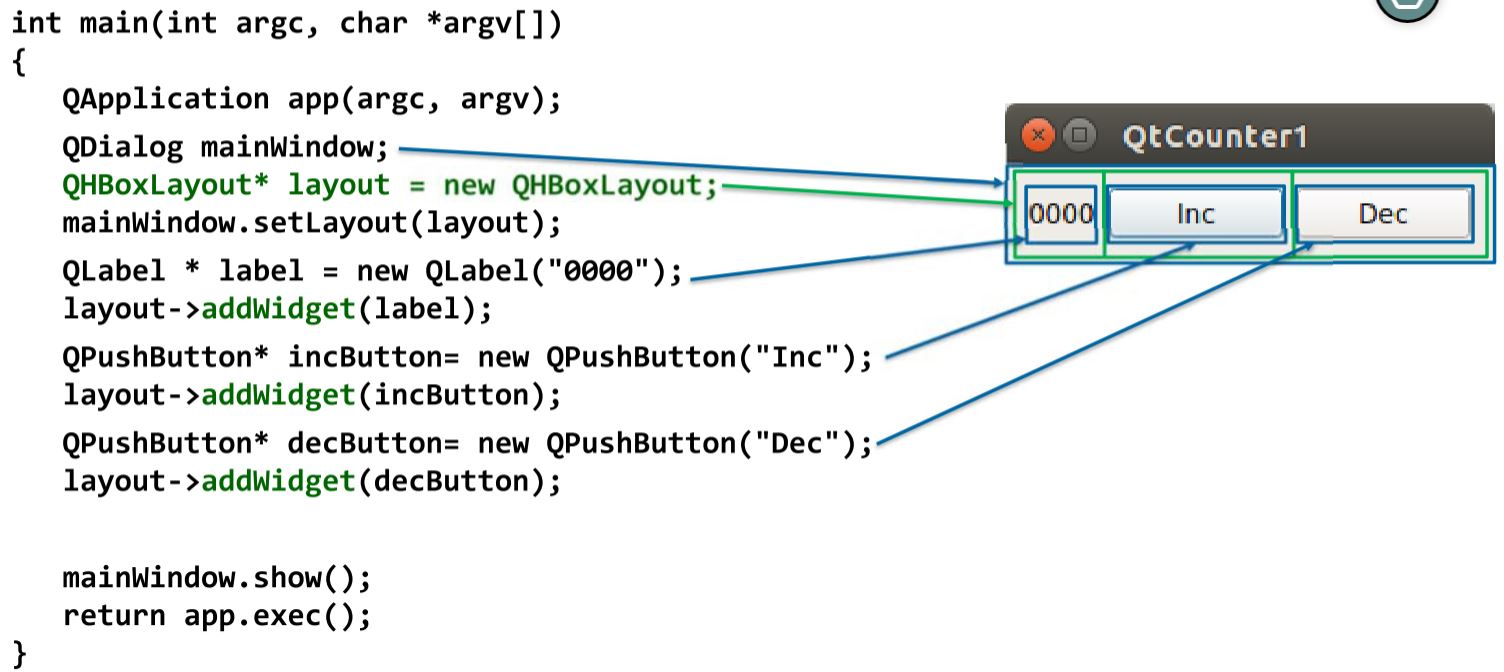
\includegraphics{Figures/QtLayoutManager}}
    \caption[]{Qt Layout Manager}
\end{figure}

Klassen, welche von QLayout ableiten:
\begin{description}[leftmargin=*, widest={\textbf{\texttt{QStackedLayout}}}]
    \item[\texttt{QHBoxLayout}] Ordnet Elemente horizontal an
    \item[\texttt{QVBoxLayout}] Ordnet Elemente vertikal an
    \item[\texttt{QGridLayout}] Ordnet Elemente in einem zweidimensionalen Gitters an
    \item[\texttt{QFormLayout}] Ordnet Elemente in Form von Zeilen an Zeile = QLabel gefolgt von anderem QWidget (z.B. QLineEdit)
    \item[\texttt{QStackedLayout}] ``Aufeinandergelegte'' Widgets (Stapel), nur immer ein Widget ist sichtbar
\end{description}


Das QLayout-Objekt ist bei einem Parent-Widget zuständig für das Layout (Anordnung) von dessen Child-Widgets:
\begin{lstlisting}[language=c++]
QDialog mainWindow;
QVBoxLayout* mainLayout = new QVBoxLayout;
mainWindow.setLayout(mainLayout);
\end{lstlisting}

Wird ein child-widget mit \lstinline{addWidget(label)} hinzugefügt, dann wird es automatisch mit dem parent Widget verknüpft.
Das QLayout-Objekt ist selbst ein ``Kind'' vom ``Parent-Widget''. Es ist zweckmässig, sich das QLayout-Objekt als ein spezielles Geschwister vorzustellen, das als Kindermädchen (``Nanny'') der ``Child-Widgets'' wirkt. QLayout-Objekte haben nie QWidget-Objekte als eigene Kinder.
Das QLayout-Objekt informiert das ``Parent-Widget'' automatisch über die Existenz der ``Child-Widgets''. Das geschieht mittels der addWidget Methode des Layout Managers:
\begin{lstlisting}[language=c++]
QLabel* label = new QLabel("0000");
mainLayout->addWidget(label);
\end{lstlisting}
Das ``Parent-Widget'' muss bei den ``Child-Widgets'' nicht explizit angegeben werden!
Layouts können auch verschachtelt werden:
\begin{lstlisting}[language=c++]
QVBoxLayout* mainLayout = new QVBoxLayout;
QHBoxLayout* bottomLayout = new QHBoxLayout;
mainLayout->addLayout(bottomLayout);
\end{lstlisting}

\subsection{Qt Layout Manager}
\begin{figure}[ht]
    \centering
    % FIXME
    % \adjustbox{width=0.7\textwidth}{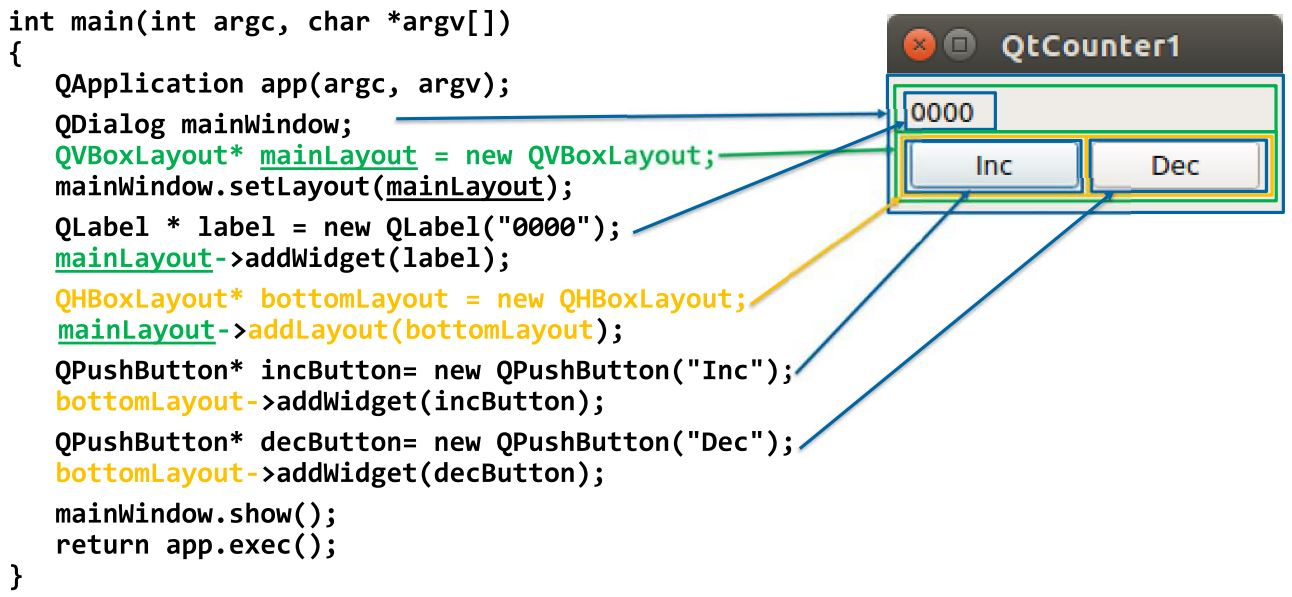
\includegraphics{Figures/layoutmitverschachtelung}}
    \caption{Qt Layout: Beispiel mit Verschachtelung}
\end{figure}

\subsection{GUI Erstellung mittels Qt-Creator}
% TODO: this does not look right
Der Zugriff auf die Widgets:
\begin{lstlisting}[language=c++]
Widget::Widget(QWidget *parent)
    : QWidget(parent)
    , ui(new Ui::Widget) // erstellt ein layout
{
    ui->setupUi(this);
    ui->lineEdit‐>setText("Test"); // Setzt den Text in lineEdit Widget
}

Widget::~Widget()
{
    delete ui; // Löscht das Layout
}
\end{lstlisting}

\subsection{Top-Level-Window/Widget}
Definition: Widgets auf der obersten Hierarchiestufe des Widget-Trees. Widgets ohne Eltern. Jedes Widget kann ein ``Top-Level-Window'' sein. Der Titelbalken (``TitleBar'') gehört nicht zu Qt! Sondern wird vom Betriebssystem erzeugt. Übliche Widgets für ``Top-Level-Windows/Widget'':
\begin{description}
    \item[\texttt{QMainWindow}] Typisch als Applikations-Window (Hauptfenster). Es hat Toolbars und eine Statusbar

    \item[\texttt{QDialog}] ``Pop-Up Window'' typisch für Abfragen wie ``Soll dies Datei wirklich gelöscht werden? Okay, Abbrechen''. Häufig modal, d.h. die Hauptanwendung bleibt blockiert, bis der Dialog beendet ist. Die Standarddialog-Klasse von Qt ist QMessageBox

    \item[\texttt{QWidget}] Einfaches Fenster, üblicherweise ``non-modal'' (d.h nicht blockierend). In den weiteren Beispielen wird meistens QWidget als Top-Level Widget verwendet
\end{description}

\section{Qt Widget Collection für Darstellungen (Selbststudium)}

%% FIXME
%%% \begin{minipage}{5cm}
%%%     \small{ Single Page Container}
%%% \end{minipage}
%%% \begin{minipage}{5cm}
%%%     \small{Multi Page Container}
%%% \end{minipage}
%%% \begin{minipage}{5cm}
%%%     \small{Button widgets}
%%% \end{minipage}
%%% 
%%%     % \adjustbox{width=5cm}{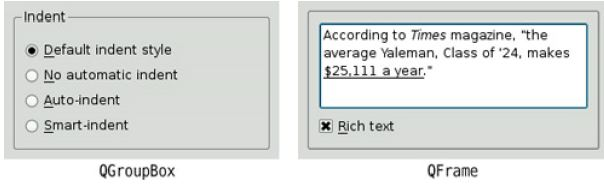
\includegraphics{Figures/scontainer}}
%%%     % \adjustbox{width=5cm}{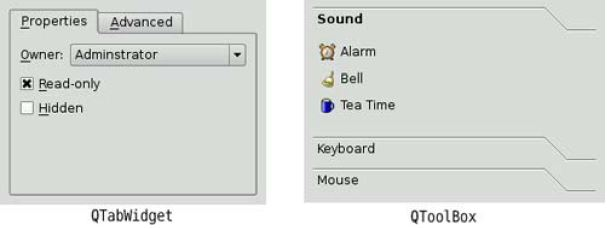
\includegraphics{Figures/mcontainer}} 
%%%     % \adjustbox{width=5cm}{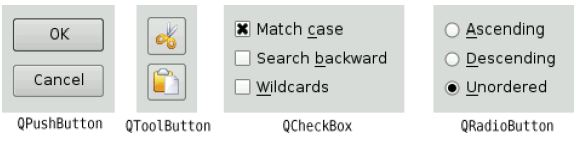
\includegraphics{Figures/buttonwidgets}}
%%% 
%%% \begin{minipage}{10cm}
%%%     \small{Input Widget}
%%% \end{minipage}
%%% \begin{minipage}{5cm}
%%%     \small{Color and Font Dialog}
%%% \end{minipage}
%%% 
%%% %   \adjustbox{width=5cm}{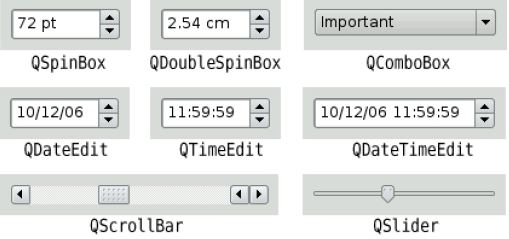
\includegraphics{Figures/inputwidget}}
%%% %   \adjustbox{width=5cm}{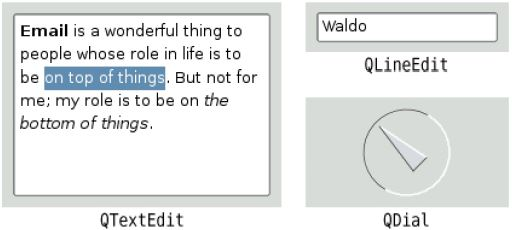
\includegraphics{Figures/inputwidget2}}
%%% %   \adjustbox{width=5cm}{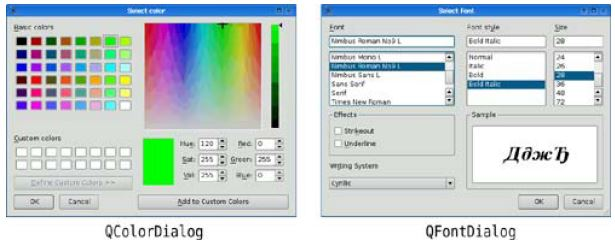
\includegraphics{Figures/cwidget}} 
%%% 
%%% \begin{minipage}{8cm}
%%%     \small{Item View Widgets}
%%% \end{minipage}
%%% \begin{minipage}{8cm}
%%%     \small{Display Widgets}
%%% \end{minipage}  
%%% 
%%%     % \adjustbox{width=8cm}{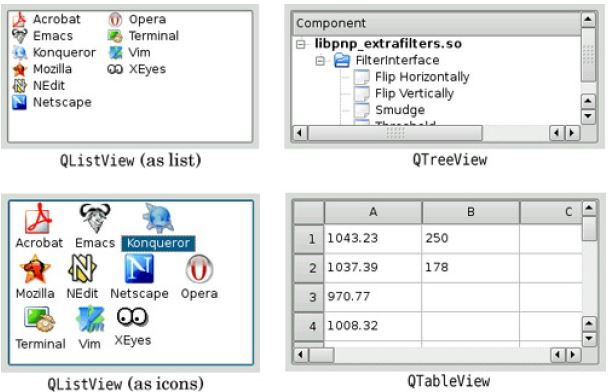
\includegraphics{Figures/vwidget}}
%%%     % \adjustbox{width=8cm}{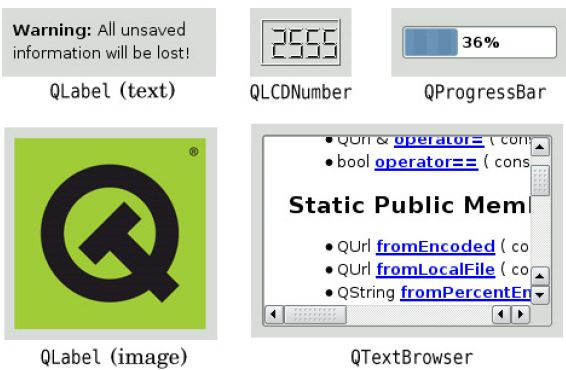
\includegraphics{Figures/dwidget}} 
%%% 
%%%     \begin{minipage}{8cm}
%%%         \small{File und Print Dialogs}
%%%     \end{minipage}
%%%     \begin{minipage}{8cm}
%%%         \small{Feedback Dialogs}
%%%     \end{minipage}  
%%% 
%%%     % \adjustbox{width=8cm}{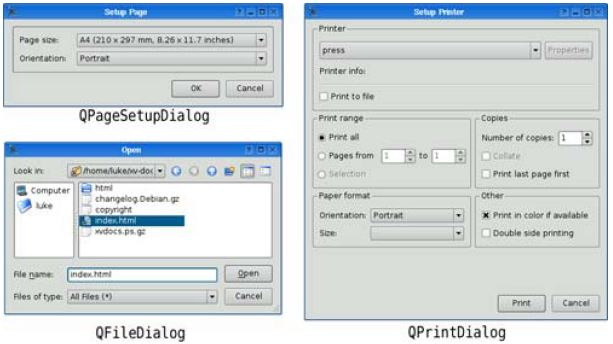
\includegraphics{Figures/pwidget}}
%%%     % \adjustbox{width=8cm}{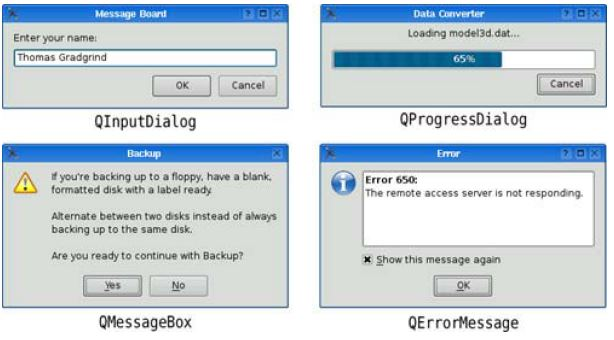
\includegraphics{Figures/fwidget}}

\section[Callbacks]{Callback, Signals und Slots - Interaktion}

\subsection{Reaktive Systeme}
Reaktive Systeme (reactive systems) reagieren auf (oft externe) Ereignisse wie digitale Inputs, die Erreichung von analogen Schwellenwerten, Timer, Buttonclicks oder ähnliches in GUI, etc. Dabei bestehen häufig auch Echtzeitanforderung an das System. Embedded Systems sind häufig auch reaktive Systeme.
Ereignisse sind per Definition asynchron, d.h. sie treten zu einem beliebigen Zeitpunkt ein, während ein ``normales'' Programm immer synchron (zuerst das, dann das, ...) ist.

\subsection{Pooling}
Ereignisse können von synchronen Programmen durch Polling verarbeitet werden, d.h. das Programm fragt periodisch oder dauernd ab, ob irgendein Ereignis eingetreten ist. Polling ist sehr einfach zu implementieren.
Dabei entstehen jedoch üblicherweise sehr viele Leerabfragen, d.h. bei vielen Abfragen ist nichts eingetreten, was eine unnötige Prozessorbelastung bewirkt. Sie können durch periodische Abfragen (Kopplung an Timer) reduziert aber nicht vermieden werden.
Die maximale Reaktionszeit wird durch die Abfrageperiode und die Anzahl Abfragen (Stichwort: Looptime bei SPS) definiert.

\subsection{C Callbacks}
Callbacks stellen bidirektionale Verbindungen von Modulen mit C dar.

\paragraph{Beispiel einer bidirektionalen Verbindung zwischen A und B} 
 Dabei kennt Klasse A, B und Klasse B kennt ebenfalls die Funktion von Klasse A.
\begin{lstlisting}[language=c]
/* file: A.c */

void aInit(void) {
    /* Eine Funktion von B wird in A aufgerufen.
     * Der Parameter der Funktion ist eine Funktion der Klasse A.
     */
    bRegisterFoo(&aFooY);  
}

void aFooY(void) {
    printf("aFooY called\n");
}
\end{lstlisting}
\begin{lstlisting}[language=c]
/* file: b.c */

static void (*regFct)(void); // Funktionspointer

void bFooX(void)
{
    if (regFct != NULL)
        regFct();
}

void bRegisterFoo(void (*fct)(void))
{
    /* Die von der Klasse A aufgerufene Funktion bRegisterFoo hat als Parameter
     * Eine Funktion aus der Klasse A, welche dem Funktionspointer regFct
     * Zugewiesen wird und wieder auf die Funktion aFooY in der Klasse A zeigt.
     */
    regFct = fct;
}
\end{lstlisting}


\paragraph{Beispiel einer unidirektionalen Verbindung zwischen Klasse A und B}
Dabei hat die Klasse A eine Verbindung zu Klasse B, aber nicht umgekehrt. Das File der Kasse A sieht folgendermassen aus: 
\begin{lstlisting}[language=c++]
#include "B.h"  // Das Header File von B wird eingefügt
class A
{
public:
    A() { b.foo();  } // Verknüpfung mit B
    void fooY() {}
private:
    B b; // Ein Objekt der Klasse B kann somit in A aufgerufen werden
};
\end{lstlisting}

\paragraph{Bidirektionale Verbindung von Klassen} 
Klasse A kennt Klasse B \emph{und} Klasse B kennt Klasse A \(\rightarrow\) Das funktioniert so nicht, da es sich um ein circular include handelt. Eine Ausnahme stellt ein Class Forwarding dar.
\begin{figure}[ht]
    % \adjustbox{width=9cm}{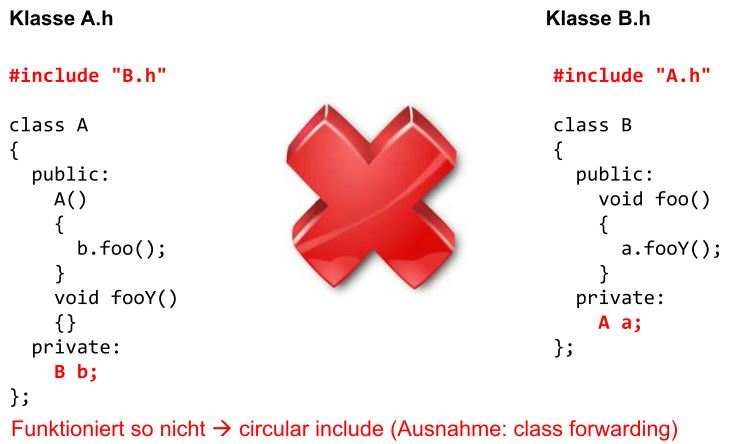
\includegraphics{Figures/bidirektional}}
    \caption{Keine gültige Bidirektionale Verbindungen von A und B}
\end{figure}

Die nachfolgenden Versionen einer bidirektionalen Verbindung:
\begin{itemize}
    \item[V1] Klasse A kennt Klasse B \emph{und} Klasse B kennt Objekt von Klasse A
        Funktioniert, da in Header-File \texttt{B.h} nur Pointer auf A, der Rest ist im \texttt{B.cpp} File. Unschön: B muss immer noch A kennen (class forwarding erforderlich). Besser: A sollte unabhängig von B sein

    \item[V2] Klasse A kennt Klasse B \emph{und} Klasse B kennt Objekt von Klasse C, Klasse A ist eine Klasse C. Bessere Variante als V1: B kennt nicht mehr A direkt

    \item[V3] Klasse A kennt Klasse B \emph{und} Klasse B kennt Objekt von Klasse C, Klasse A ist eine Klasse C. Besser Variante als V2: der Funktionspointer wird weggelassen, da überflüssig
\end{itemize}

\begin{figure}[ht]
% FIXME
% \adjustbox{width=12cm}{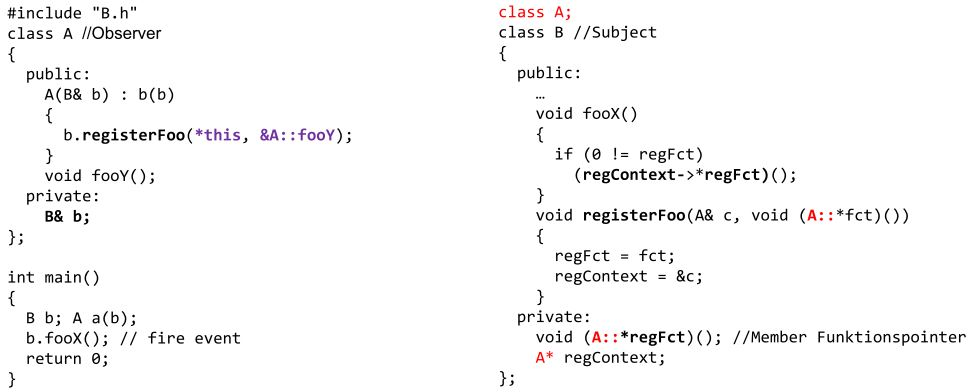
\includegraphics{Figures/bidirektionalv1}}
% \adjustbox{width=12cm}{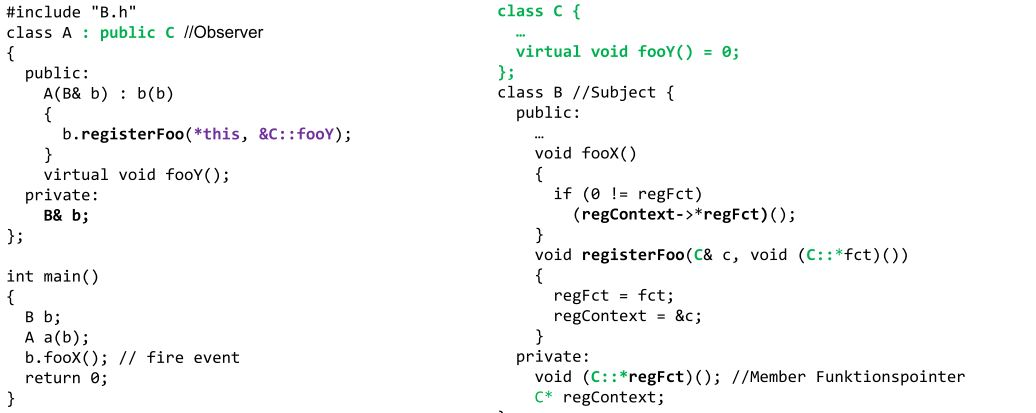
\includegraphics{Figures/bidirektionalv2}}
% \adjustbox{width=12cm}{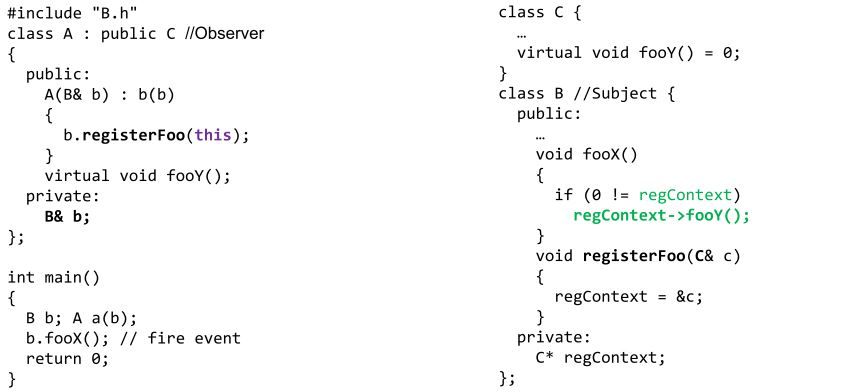
\includegraphics{Figures/bidirektionalv3}}
\caption[]{Bidirektionale Verbindungen: V1-V3}
\end{figure}

Abstraktere C++ Umsetzungen folgen im Modul OOAD: Observer Pattern.
Die kennengelernten Callback und Observer Methoden können für native C++ verwendet werden. In Qt können Signal/Slots verwendet werden.

\section[Qt signals and slots]{Qt Signals and Slots: Interaktion zwischen QObjects}

Qt verwendet anstatt Callbacks ein Signal-Slot Prinzip. Analogie zu Callbacks: Das zu informierende Objekt (Observer) hat einen slot, Das informierende Objekte (Subject) hat ein signal, die Registrierung erfolgt über eine connect Funktion. 

Es wird der Funktionspointer von C++--Member verwendet. Signals und Slots werden mit dem \lstinline{QObject::connect()} verbunden. Form:
\begin{lstlisting}[language=c++]
connect(
    SenderObj*,       // Subject
    SenderMethode*,   // Signal1
    EmpfängerObj*,    // Observer
    EmpfängerMethode* // Slot2
);
\end{lstlisting}
Beispiel: \lstinline{connect(&b, &B::fooX, &a, &A::fooY);}

\begin{figure}[ht]
    \centering
    % \adjustbox{width=0.9\textwidth}{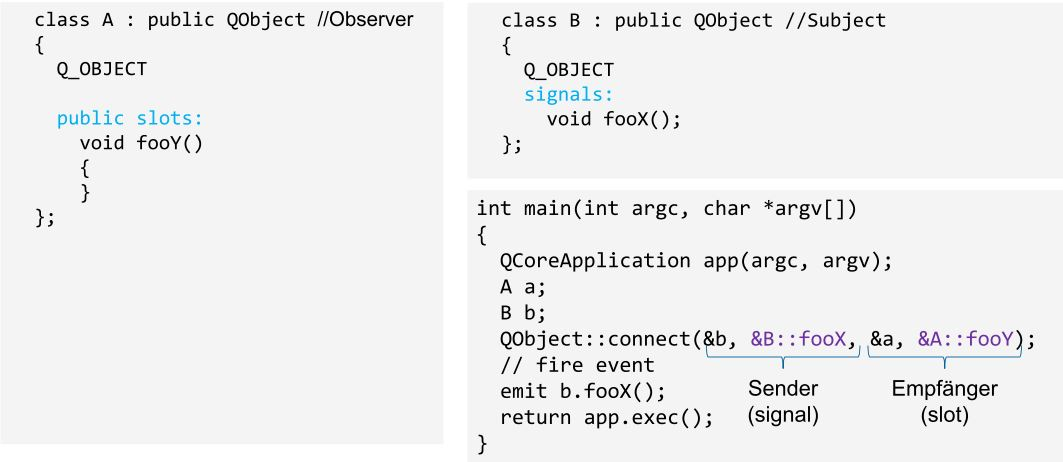
\includegraphics{Figures/bspsignal}}
    \caption{Beispiel Signal \& Slots}
\end{figure}

%\begin{figure}[ht]
%   \centering
%   \adjustbox{width=0.9\textwidth}{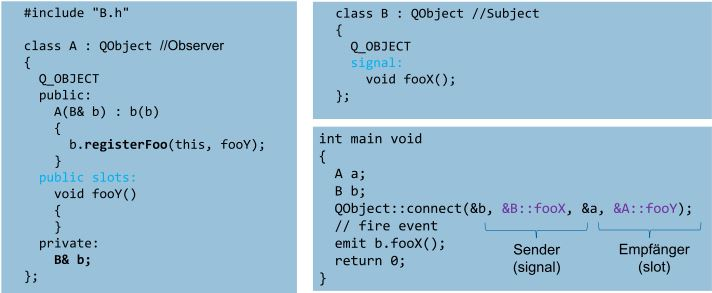
\includegraphics{Figures/bspsigslot}}
%   \caption[]{Beispiel Signal \& Slots}
%\end{figure}

\subsection[Signals]{Signals: Signal-Memberfunktion}
Signals werden nur deklariert und nicht implementiert. Es werden keine Zugriffsrechte wie private public oder protect verwendet. Der Rückgabetyp ist immer void. Ein Signalaufruf erfolgt mit \lstinline{emit method(value)}. Die C++ Definition erfolgt mit \lstinline{#define signals public}. Ein Signal kann mit mehreren Slots oder anderen Signalen verbunden werden. Mehrere Signal können mit demselben Slot verbunden werden. Es kann einen Übergabeparameter haben.

\subsection{Slots}
Slots sind immer public (by default). Für private slots muss das Keyword slots weggelassen werden. Die C++ Definition lautet \lstinline{#define slots}. Slots können einen Übergabeparameter haben.

\subsection{Signals \& Slots: Connect}

Der Parameter Typ und Anzahl muss stimmen
\begin{center}
    \begin{tabular}{l l}
        Signal                                 & Slot \\
        \midrule
        \texttt{void clicked()}             & \texttt{void onClicked()} \\
        \texttt{void indexChanged(int idx)} & \texttt{void onIndexChanged(int idx)}
    \end{tabular}
\end{center}


\subsubsection*{Ab Qt5 -- mit Funktionspointer}
\begin{lstlisting}[language=c++]
connect(senderObj, &SenderClass::senderMethod, revObj, &RevClass:revMethod);
\end{lstlisting}
\begin{itemize}
    \item weniger Klammern 
    \item keine Datentypen für Parameter; aber Compiler meldet Fehler
\end{itemize}

\subsubsection*{Alte Notation}
Keine Compilerfehlermeldungen, falls falsch: wird zur Laufzeit geprüft
\begin{lstlisting}[language=c++]
connect(button, SIGNAL(clicked()), count, SLOT(incValue()));
\end{lstlisting}

\subsubsection*{Globale Funktionen als Slots (ab Qt5)} 
\begin{lstlisting}[language=c++]
void printValue(int x)
{
    std::count << "Value=" << x << std::endl;
} 

connect(button, &QPushButton::clicked, &printValue); 
\end{lstlisting}


\subsubsection*{Überladene Methoden} 
\begin{lstlisting}[language=c++]
void QLabel::setNum(int num)
void QLabel::setNum(double num)
connect(..., static_cast<void (QLabel::*)(int)>(&QLabel::setNum), ..., ...);
\end{lstlisting}

\begin{figure}[ht]
    \centering
    % \adjustbox{width=0.7\textwidth}{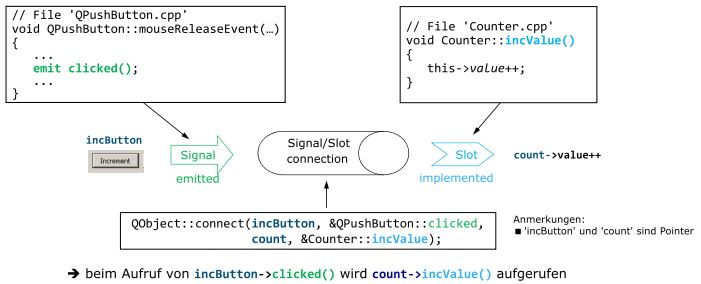
\includegraphics{Figures/sigausframework}}
    \caption{Beispiel mit Signal aus Framework}
\end{figure}

\begin{figure}[ht]
    \centering
    % \adjustbox{width=0.7\textwidth}{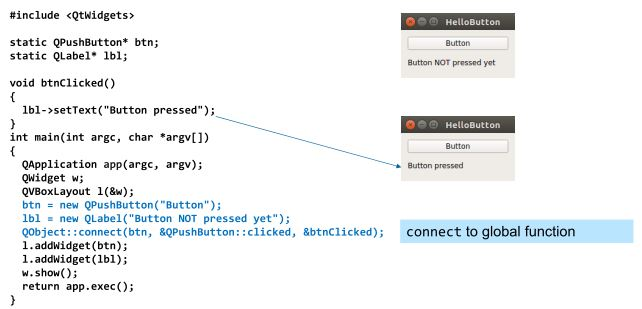
\includegraphics{Figures/hellobutton}}
    \caption{``Hello Button'' - GUI Programm}
\end{figure}

\begin{figure}[ht]
    \centering
    % \adjustbox{width=9cm}{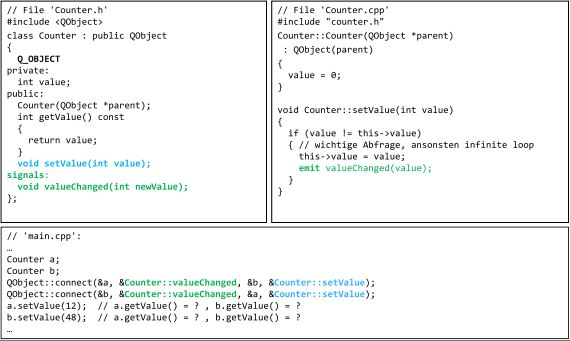
\includegraphics{Figures/selfconnect}}
    \caption{Counter Beispiel: Connect mit sich selbst}
\end{figure}


